\section{Ester - Lipid}
\begin{Muctieu}
	\begin{itemize}
		\item  Nêu được khái niệm về lipid, chất béo, acid béo, đặc điểm cấu tạo phân tử ester.
		\item  Viết được công thức cấu tạo và gọi được tên một số ester đơn giản (số nguyên tử C trong phân tử $\leq 5$ ) và thường gặp.
		\item  Trình bày được đặc điểm về tính chất vật lí và tính chất hoá học cơ bản của ester (phản ứng thuỷ phân) và của chất béo (phản ứng hydrogen hoá chất béo lỏng, phản ứng oxi hoá chất béo bởi oxygen không khí).
		\item  Trình bày được phương pháp điểu chế ester và ứng dụng của một số ester.
		\item  Trình bày được ứng dụng của chất béo và acid béo (omega-3 và omega-6).
	\end{itemize}
\end{Muctieu}
\Noibat[\maunhan][\LARGE\bfseries\fontfamily{qag}\selectfont][\faBeer]{Nội dung bài học}
\subsection{ESTE}
\subsubsection{Khái niệm}
\columnratio{0.7}
%%==============Đường phân cách hai cột===========================%%%
\setlength{\columnseprule}{0pt}
\begin{paracol}{2}
	Khi ta thay thế nhóm OH trong axit cacboxylic bằng nhóm OH ta thu được este.
	\begin{center}
		\schemestart 
		\chemname{\chemfig{R-C(=[::-90]O)-@{a}{OH}}}{\color{\mycolor!40!black}{Axitcacboxylic}}
		\chemmove{\nodefill[\maunhan]{a}{a}}
		\arrow(.mid east--.mid west){->[\scriptsize{thay nhóm OH}][\scriptsize{bằng nhóm  OR}][0pt]}[0,1.5,,]
		\chemname{\chemfig{R-C(=[::-90]O)-@{b}{OR}}}{\color{\mycolor!40!black}{Este}}
		\chemmove{
		\nodefill[\maunhan]{b}{b}
		}		
		\schemestop
	\end{center}
	Trong đó: R,R' có thể thuộc loại: no (không chứa liên kết pi) ; không no (chứa liên kết $ \pi $ linh động) hoặc thơm (chứa vòng benzen)
	
	\begin{itemize}
		\item Nếu R và R' đều no: este  no.
		\item Nếu R hoặc R' đều no: este không no.
		\item Nếu R hoặc R' đều no: este thơm.
	\end{itemize}
	Nhóm COO được xem là nhóm chức của este.
	\switchcolumn
	\textbf{Ví dụ:}\\ Este: \chemfig{CH_3COOC_2H_5}\\
	\textbf{Ví dụ:}\\
	\resizebox{!}{3.3cm}{%
		\setlength{\tabcolsep}{4pt}
		\begin{tabular}{|r|c|}
			\hline
			\chemfig{HCOOCH_3} & \multirow{2}{*}{ este no} \\
			\cline{1-1}
			\chemfig{CH_3COOC_2H_5} &  \\
			\hline
			\chemfig{CH_2=CHCOOCH_3} &  \multirow{3}{*}{ \makecell{este\\ không no} } \\
			\cline{1-1}
			\chemfig{C_2H_5COOCH=CH_2} &  \\
			\cline{1-1}
			\chemfig{CH_2=CHCOOCH=CH_2} &  \\
			\hline	
			\makecell[r]{%
				~	\\
				\chemfig{[:-30]**6(---(-COOCH_3)---)}\\
				~
			} & \multirow{4}{*}{\makecell[c]{este thơm}}  \\
			\cline{1-1}
			\makecell[r]{%
				~	\\
				\chemfig{CH_3COO-[:0]**6(------)}\\
				~
			}& \\
			\hline	
		\end{tabular}
	}
\end{paracol}
\begin{note}
	\begin{itemize}
		\item Este đơn chức có một nhóm COO.
		Công thức tổng quát của este no, đơn chức, mạch hở:\chemfig{C_mH_{2m+1}COOC_pH_{2p+1}}\\ ( $ m\geq 0,p \geq 1 $)\\
		Hay \chemfig {C_nH_{2n}O_2}
		\item Este đa chức: có 2 nhóm COO trở lên.
	\end{itemize}
\end{note}
\subsubsection{Danh pháp}
\begin{center}
	\tcbox[tcbox width=auto,fontupper=\bfseries\fontfamily{qag}\selectfont,size=small,
	on line,before upper=\strut,
	colframe=\mycolor!75!black,
	colback=\mycolor!5!white]{Tên este RCOOR' = Tên gốc R' + Tên gốc axit RCOO}
\end{center}
\vspace*{0.5cm}
\columnratio{0.5}
\begin{paracol}{2}
	\begin{table}
		\centering\caption{\textbf{Tên một số gốc hiđrocacbon thường gặp}}\label{tab:gocHC}
		\resizebox{8cm}{!}{
			\begin{tabular}{|C{1.2cm}|l|l|l|}
				\hline
				\thead{\sffamily\textbf{\makecell{Phân  \\loại}}}
				& 
				\multicolumn{2}{c|}{\thead{\sffamily\textbf{Gốc hiđrocacbon}}} & 
				\thead{\sffamily\textbf{Tên gọi}}\\
				\hline
				\multirow{6}{*}{ No} & \multicolumn{2}{l|}{\chemfig{CH_3-[,0.8]}} & metyl\\
				
				& \multicolumn{2}{l|}{\chemfig{C_2H_5-[,0.8]}} & etyl\\
				\cline{2-4}
				& \multirow{2}{*}{ \chemfig{C_3H_7-[,0.8]}} & \chemfig{CH_3CH_2CH_2-[,0.8]}& propyl\\
				
				&  & \chemfig{{(CH_3)}_2CH-[,0.8]} & isopropyl\\
				\cline{2-4}
				& \multicolumn{2}{l|}{\chemfig{CH_3CH_2CH_2CH_2-[,0.8]}} & butyl\\
				
				& \multicolumn{2}{l|}{\chemfig{{(CH_3)}_2CHCH_2CH_2-[,0.8]}} & isoamyl\\
				\hline
				\multirow{2}{*}{\makecell{Không\\ No}}& \multicolumn{2}{l|}{\chemfig{CH_2=CH-[,0.8]}} & vinyl\\
				
				& \multicolumn{2}{l|}{\chemfig{CH_2=CHCH_2-[,0.8]}} & anlyll\\
				\hline
				
				\multirow{4}{*}{Thơm}&\multicolumn{2}{l|}{\makecell[l]{~\\\small\chemfig{[:-30]**6(---(-)---)}\\~\\}} & phenyl\\
				
				& \multicolumn{2}{l|}{\makecell[l]{~\\\small\chemfig{[:-30]**6(---(-CH_2-)----)}\\~\\}} & benzyl\\
				\hline
			\end{tabular}
		}
	\end{table}
	\switchcolumn
	\centering
	{\textbf{Chú ý:Một số este thường gặp}}
	\resizebox{8.6cm}{!}{
		\begin{tabular}{|ll|}
			\hline
			\thead{\sffamily\textbf{Công thức cấu tạo}} & \thead{\sffamily\textbf{Tên gọi}} \\
			\hline
			\chemfig{HCOOCH_3} & metyl fomat \\
			\chemfig{HCOOC_2H_5} & etyl fomat \\
			\chemfig{HCOOCH_2CH_2CH_3} & propyl fomat \\
			\chemfig{[,,6,1,,]HCOOCH([:-90,,5,1,,]-CH_3)-CH_3} & isopropyl fomat \\
			\chemfig{CH_3COOCH_3} & metyl axetat \\
			\chemfig{CH_3COOC_2H_5} & etyl axetat \\
			\chemfig{CH_3COOCH_2CH_2CH{(CH_3)}_2} & isoamyl axetat \\
			\chemfig{CH_3COOCH=CH_2} & vinyl axetat \\
			\chemfig{CH_2=CH-COOCH_3} & metyl acrylat \\
			\chemfig{CH_2=CH([:-90,,1,1,,]-CH_3)-COOCH_3} & metyl metacrylat \\
			\makecell[l]{%
				~\\
				\chemfig{CH_3COOCH_2-**6(------)}\\
				~\\
			} & benzyl axetat \\
			\hline
		\end{tabular}
	}
\end{paracol}

\begin{table}
	\begin{center}
		\caption{\textbf{Tên một số gốc axit tương ứng thường gặp}}\label{tab:gocAx}
	\end{center}
	\begin{center}
		\begin{tabular}{|c|l|c|}
			\hline
			\multirow{2}{*}{\thead{\sffamily\textbf{Phân loại}}} & \multicolumn{2}{c|}{\sffamily\textbf{Gốc axit}} \\
			\cline{2-3}
			& \thead{Công thức} & \thead{Tên gọi}\\
			\hline
			\multirow{4}{*}{No}& \chemfig{HCOO-} & fomat\\
			& \chemfig{CH_3COO-} & axetat\\
			& \chemfig{C_2H_5COO-} & propionat\\
			& \chemfig{CH_3CH_2CH_2COO-} & butyrat\\
			\hline
			\multirow{3}{*}{Không No}& \chemfig{CH_2=CHCOO-} & acrylat\\
			& \chemfig{CH_2=C([:-90]-CH_3)([:90]-CH_3)-COO-} & metacrylat\\
			\hline
			Thơm		& \makecell[l]{%
				~\\
				\chemfig{[:-30]**6(---(-COO-)---)}\\
				~\\
			} & benzoat\\
			\hline
		\end{tabular}
	\end{center}
\end{table}
%%%=========Tinh chat vat ly=========%%%
\subsubsection{Tính chất vật lý}
\begin{tomtat}
	\begin{multicols}{2}
		\begin{itemize}
			\item Trạng thái ở đều kiện thường: chất lỏng hoặc rắn
			\item Nhiệt độ nóng chảy và nhiệt độ sôi: Thấp hơn so với ancol và axit cacboxylic có số nguyên tử cacbon và số nhóm chức tương đương.
			\item Tính tan: không tan trong nước, tan nhiều trong dung môi hữu cơ.
			\item Nhiều este có mùi thơm của hoa quả chín
		\end{itemize}
		\columnbreak % chuyển nội dung sang cột khác
		%	\newcolumn Có thể dùng lệnh này để chuyển sang cột khác
		\begin{center}
			{\textbf{Một số este tạo hương vị\\ đặc trưng cho hoa quả}}
		\end{center}
		\begin{center}
			\begin{tabular}{|ll|}
				\hline
				\thead{\sffamily\textbf{Este}} & \thead{\sffamily\textbf{Mùi}} \\
				\hline
				\chemfig{HCOOCH_3} & táo chín \\
				\chemfig{HCOOC_2H_5} & đào chín \\
				\chemfig{CH_3COOC_2H_5} & bơ \\
				\chemfig{CH_3COOCH_2CH_2CH{(CH_3)}_2} & chuối chín \\
				\hline
				\chemfig{C_2H_5COOC_2H_5} & \multirow{2}{*}{dứa} \\
				\chemfig{C_3H_7COOC_2H_5} &  \\
				\hline
				\makecell[l]{%
					~\\
					\chemfig{CH_3COOCH_2-**6(------)}\\
					~\\
				} & hoa nhài \\
				\hline
			\end{tabular}
		\end{center}
	\end{multicols}
\end{tomtat}
\subsubsection{Tính chất hóa học}
\paragraph{Phản ứng thủy phân trong môi trường axit}
\begin{center}
	\schemestart
	\chemfig{RCOOR'}
	\+
	\chemfig{H_2O}
	\arrow{<=>[$\scriptsize t^\circ $][$H_2{SO_4}_\text{đặc} $]}[,1.5,,\mycolor,-latex]
	\chemfig{RCOOH}
	\+
	\chemfig{R'OH}
	\schemestop
\end{center}
\begin{itemize}
	\item \textbf{Đặc điểm:} phản ứng thuận nghịch
\end{itemize}
\paragraph{Phản ứng thủy phân trong môi trường bazơ}
\begin{center}
	\schemestart
	\chemfig{RCOOR'}
	\+
	\chemfig{NaOH}
	\arrow{->[$\scriptsize t^\circ $][]}[,1.5,,\mycolor,-latex]
	\chemfig{RCOONa}
	\+
	\chemfig{R'OH}
	\schemestop
\end{center}
\begin{itemize}
	\item \textbf{Đặc điểm:} phản ứng một chiều
	\item \textbf{Tên gọi:} Phản ứng xà phòng hóa
\end{itemize}
\paragraph{Phản ứng cộng và phản ứng trùng hợp của este không no}
\columnratio{0.3}
\begin{paracol}{2}
	\begin{itemize}
		\item Các este không no có thể tham gia phản ứng cộng \chemfig{H_{2}}(xúc tác, $ t^\circ $), cộng \chemfig{Br_{2}}, cộng HX(X là gốc axit) và phản ứng trùng hợp.
		\item Một số este đơn giản có liên kết C=C tham gia phản ứng trùng hợp giống như anken.
	\end{itemize}
	\switchcolumn
	\textbf{Ví dụ 1:}\\
	\schemestart 
	\chemfig{CH_{2}=CHCOOCH_{3}}
	\+
	\chemfig{H_{2}}
	\arrow{->[$ t^\circ $][Ni][]}[,1,,]
	\chemfig{CH_{3}CH_{2}COOCH_{3}}
	\schemestop
	\\
	\textbf{Ví dụ 2:}\\
	\schemestart 
	\chemfig{CH_{2}=CHCOOCH_{3}}
	\+
	\chemfig{Br_{2}}
	\arrow{->[$ t^\circ $][Ni][]}[,1,,]
	\chemfig{CH_{2}BrCHBrCOOCH_{3}}
	\schemestop
	\\
	\textbf{Ví dụ 3:}\\
	\schemestart 
	\chemname{\chemfig{nCH_{2}=CH-C(=[:-90]O)-O-CH_{3}}}{metyl acrylat}
	\arrow(.mid east--.mid west){->[\scriptsize{xt, $ t^\circ$}][][]}[,1,,]
	\chemname{%
		\chemfig{%
			\vphantom{CH_2}-[@{left,.75}]CH(-[:-90]COOCH_{3})-CH_{2}-[@{right,.25}]
		}
		\polymerdelim[%
		height = 6pt,
		indice = \!\!n,
		depth = 15pt,
		]{left}{right}
	}
	{poli(metyl acrylat)}
	\schemestop
\end{paracol}

\paragraph{Phản ứng cháy}
\begin{paracol}{2}
	\begin{itemize}
		\item Các este dễ cháy và tỏa nhiều nhiệt:
	\end{itemize}
	\switchcolumn
	\textbf{Ví dụ 4:}\\
	\schemestart 
	\chemfig{CH_{3}COOC_{2}H_{5}}
	\+
	\chemfig{5O_{2}}
	\arrow{->[$ t^\circ $][][]}[,1,,]
	\chemfig{4CO_{2}}
	\+
	\chemfig{4H_{2}O}
	\schemestop
\end{paracol}
\begin{note}
	R'OH sinh ra có thể phản ứng với môi trường (nếu là phenol) hoặc không bền chuyền hóa thành anđehit, xeton.
	\begin{itemize}
		\item Este $+\mathrm{NaOH} \rightarrow$ Muối + anđehit:\par
		\schemestart
		\chemfig{RCOOCH=CHR'}
		\+
		\chemfig{NaOH}
		\arrow{->[$ t^\circ $][][]}[0,.7,,]
		\chemfig{RCOONa}
		\+
		\chemfig{R'CH_2CHO}
		\schemestop
		
		\item Este $+\mathrm{NaOH} \rightarrow$ Muối + xeton:\par
		\schemestart
		\chemfig{RCOOC(-[:-90,,5,1,,]R'')=CHR'}
		\+
		\chemfig{NaOH}
		\arrow(.mid east--.mid west){->[$ t^\circ $][][]}[0,.7,,]
		\chemfig{RCOONa}
		\+
		\chemfig{R'CH_2C(=[:-90,,4,1,,]O)-R''}
		\schemestop
		\item Este $+\mathrm{NaOH} \rightarrow 2 \mathrm{\text{Muối}}+\mathrm{H}_2 \mathrm{O}$:\par
		\resizebox{14.5cm}{!}{\schemestart
			\chemfig{RCOO-**6(---(-R')---)}
			\+
			\chemfig{2NaOH}
			\arrow{->[$ t^\circ $][][]}[0,.7,,]
			\chemfig{RCOONa}
			\+
			\chemfig{R'-**6(---(-ONa)---)}
			\+
			\chemfig{H_2O}
			\schemestop}
	\end{itemize}
\end{note}
\subsubsection{Điều chế và ứng dụng}
\paragraph{Điều chế}

\Noibat[\maunhan][][\faStar][]{Este của ancol}
\begin{itemize}
	\item \textbf{Phương pháp:} Đun hồi lưu ancol với axit hữu cơ
	\item Dùng \chemfig{H_{2}SO_{4}} vừa làm chất xúc tác vừa làm chất hút nước để tăng hiệu suất phản ứng.
\end{itemize}
\begin{center}
	\schemestart 
	\chemname[-0.5cm]{\chemfig{CH_{3}COOH}}{axetic acid}
	\+
	\chemname[-0.5cm]{\chemfig{{(CH_{3})}_{2}CHCH_{2}CH_{2}OH}}{ancol isoamylic}
	\arrow(.mid east--.mid west){<=>[\scriptsize$ t^\circ $][\scriptsize\chemfig{H_2SO_4}][]}[,1,,]
	\chemname[-0.5cm]{\chemfig{CH_{3}COOCH_2CH_2CH{(CH_3)}_2}}{isoamyl axetat}
	\+
	\chemname[-0.5cm]{\chemfig{H_2O}}{nước}
	\schemestop
\end{center}

\Noibat[\maunhan][][\faStar][]{Este của phenol}:
\begin{itemize}
	\item \textbf{Phương pháp:} Dùng anhidrit axit tác dụng với phenol và phản ứng xảy ra một chiều.
	\item \textbf{Chú ý:}: không dùng phenol tác dụng với axit cacboxylic
\end{itemize}

\begin{center}
	\resizebox{15cm}{!}{
		\schemestart 
		\chemfig{[:-30]**6(---(-OH)---)}
		\+
		\chemname{\chemfig{CH_3-C(=[:-90]O)-O-C(=[:-90]O)-CH_3}}{anhiđrit axit}
		\arrow(.mid east--.mid west){->[][][]}[,1,,]
		\chemname{\chemfig{CH_{3}COO-**6(------)}}{phenyl axetat}
		\+
		\chemfig{CH_{3}COOH}
		\schemestop
	}
\end{center}
\paragraph{Ứng dụng}
\begin{itemize}
	\item 	Công nghiệp hương liệu và mùi hương 
	\item 	Ngành thực phẩm , đồ uống và mỹ phẩm
	\item   Công nghiệp sơn và mực in
	\item   Dược phẩm
\end{itemize}
\hspace*{2.5cm}
\resizebox{!}{11cm}{%
	\begin{tikzpicture}[declare function={d=5cm;}]
		\path 
		(0,0) coordinate (O)
		(d,0) coordinate (A)
		($ (O)!1!90:(A) $) coordinate (B)
		($ (O)!1!180:(A) $) coordinate (C)
		($ (O)!1!270:(A) $) coordinate (D)
		;
		\begin{scope}
			\clip (A) coordinate (E)  circle (2.3);
			\path (E) 	node(Et){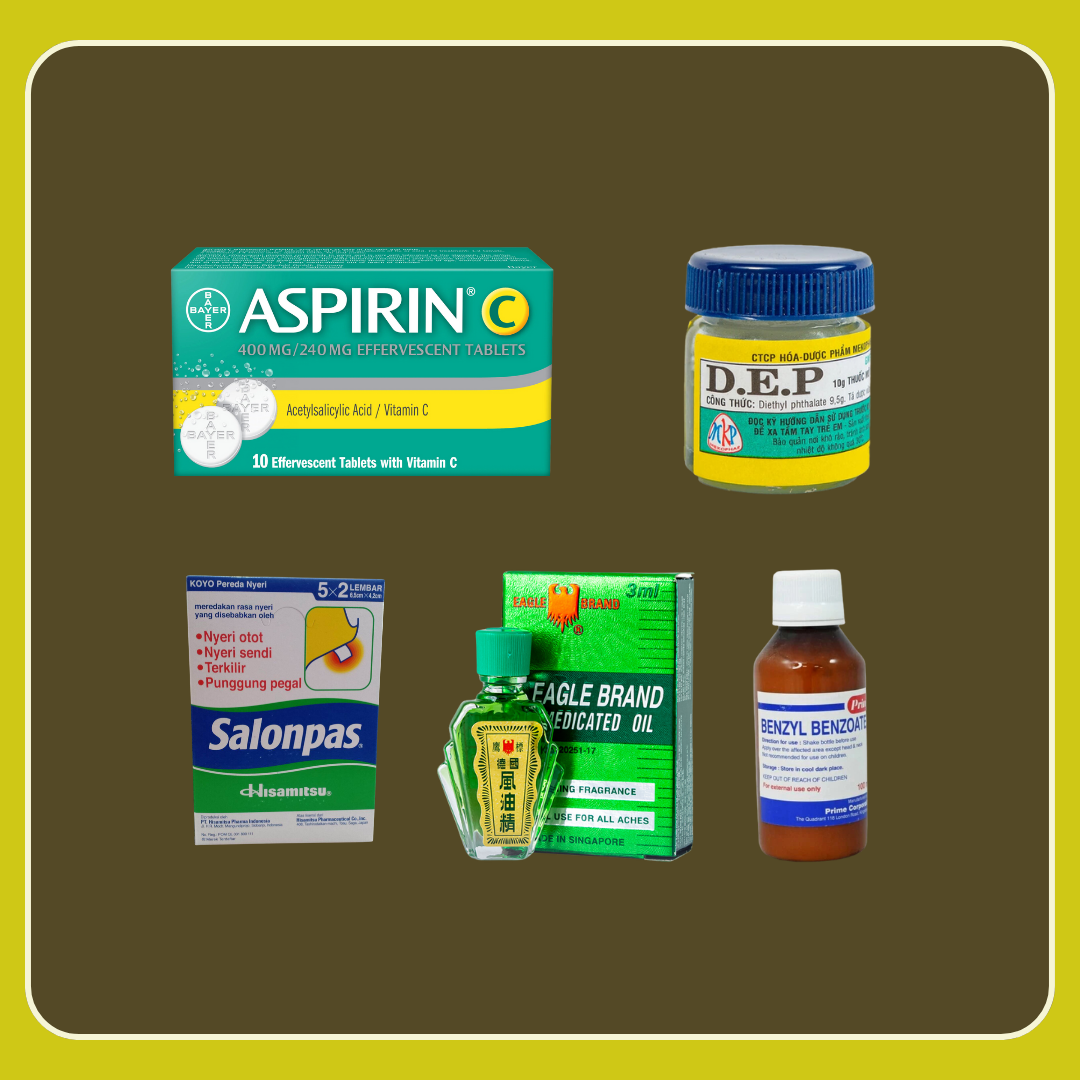
\includegraphics[width=5cm]{Images/anhhoahoc12/duocpham.png}};
			\draw[\mycolor,line width=3pt] (E) circle (2.3);
		\end{scope}
		\path (Et.south) 		node[anchor=north,\mycolor!50!black,font=\fontsize{14pt}{6pt}\bfseries\sffamily]{Dược phẩm}
		;
		\begin{scope}
			\clip (B) coordinate (F)  circle (2.3);
			\path (F) 
			node (Ft) {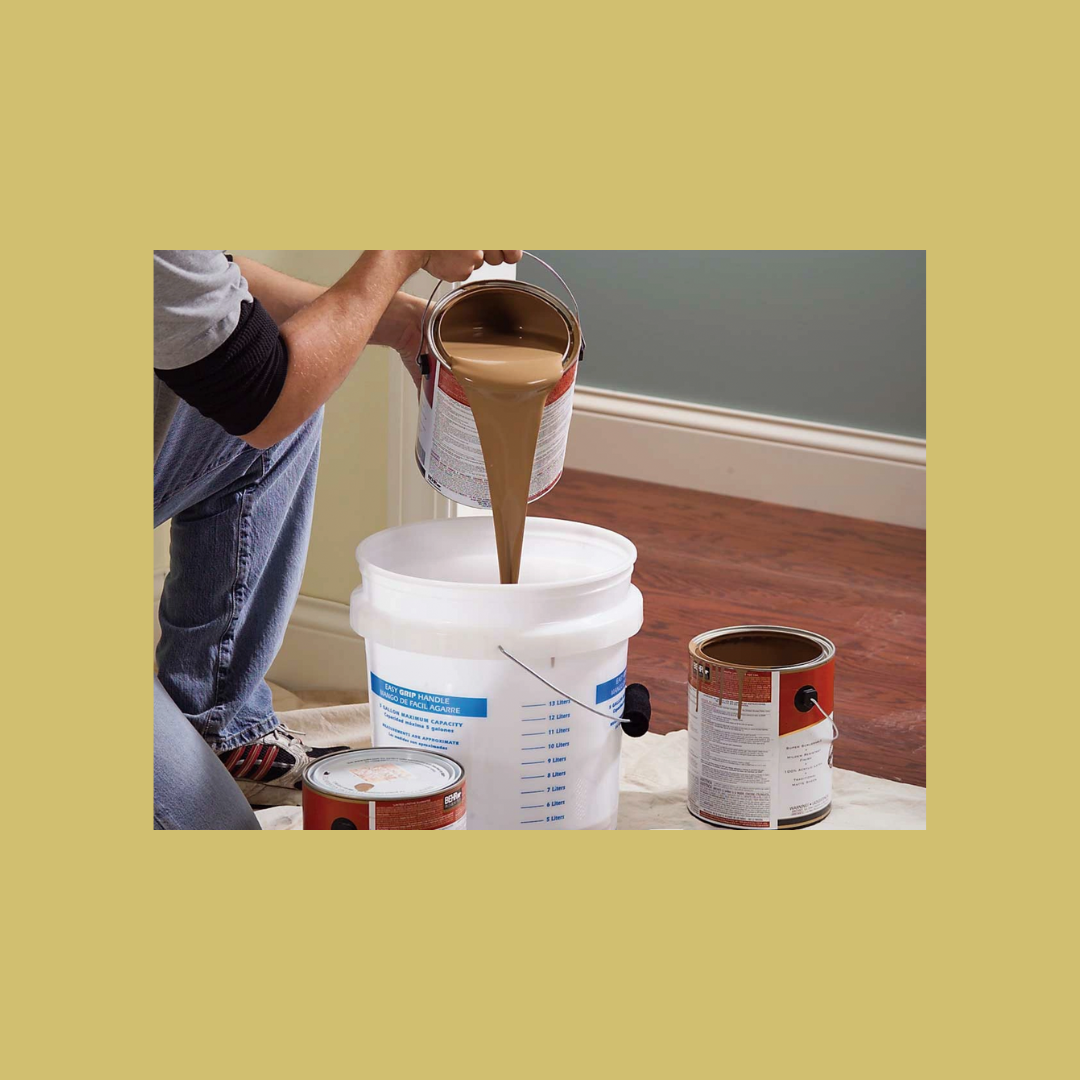
\includegraphics[width=5cm]{Images/anhhoahoc12/son.png}}
			;
			\draw[\mycolor,line width=3pt] (F) circle (2.3);
		\end{scope}
		\path (Ft.east) 		node[anchor=west,\mycolor!50!black,font=\fontsize{14pt}{6pt}\bfseries\sffamily]{Pha sơn,\\ mực in}
		;
		\begin{scope}
			\clip (C) coordinate (G)  circle (2.3);
			\path (G) node(Gt){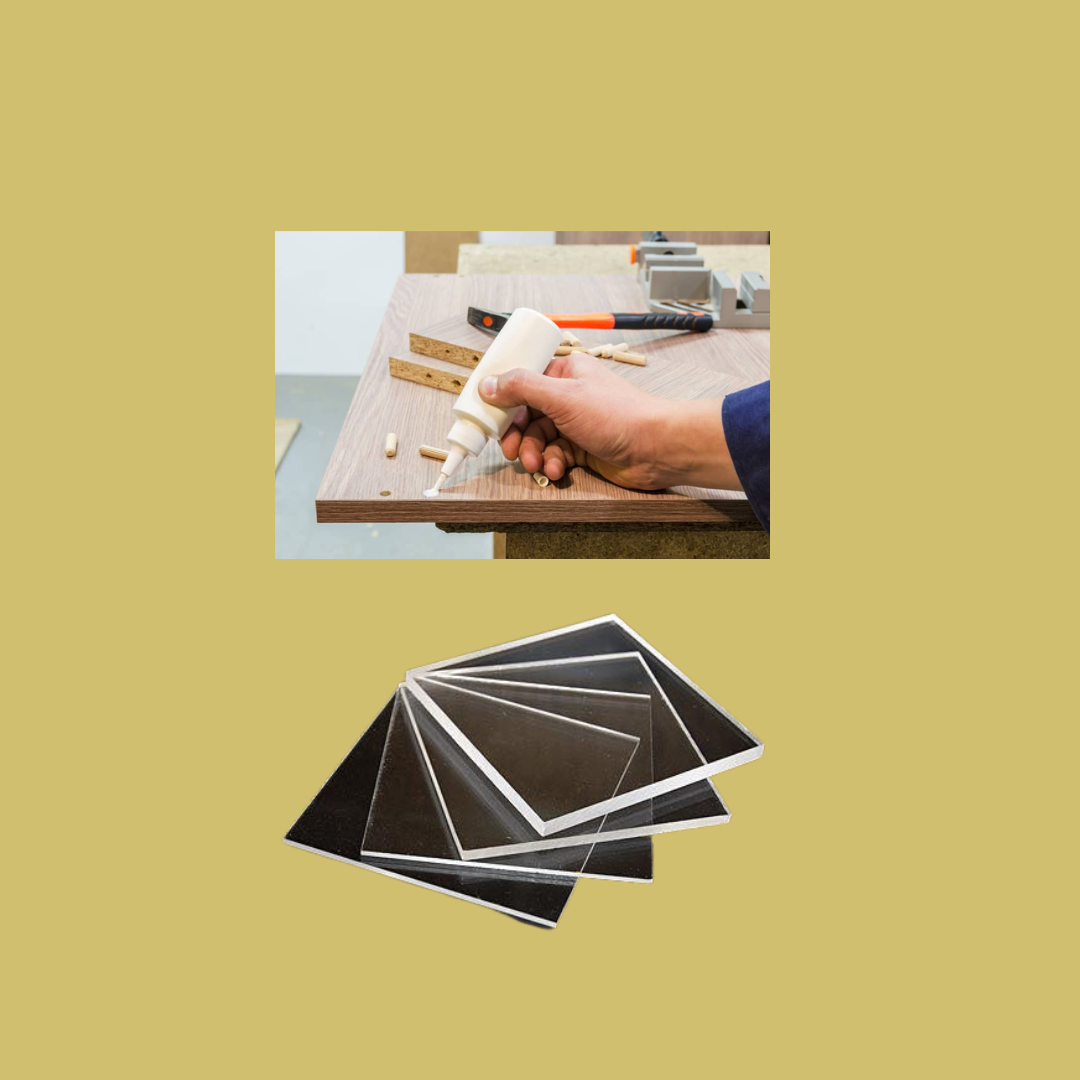
\includegraphics[width=5cm]{Images/anhhoahoc12/chatdeo.png}};
			\draw[\mycolor,line width=3pt] (G) circle (2.3);
		\end{scope}
		\path (Gt.north) 		node[anchor=south,\mycolor!50!black,font=\fontsize{14pt}{6pt}\bfseries\sffamily]{Chất dẻo,\\thủy tinh hữu cơ}
		;
		\begin{scope}
			\clip (D) coordinate (H)  circle (2.3);
			\path (H) node(Ht){
\includegraphics[width=5cm]{Images/anhhoahoc12/mypham.png}};
			\draw[\mycolor,line width=3pt] (H) circle (2.3);
		\end{scope}
		\path (Ht.west) 		node[anchor=east,\mycolor!50!black,font=\fontsize{14pt}{6pt}\bfseries\sffamily]{Hương liệu,\\mỹ phẩm}
		;
	\end{tikzpicture}}
\subsection{LIPID}
	\subsubsection{Khái niệm về lipid, chất béo, acid béo}
	\begin{tomtat}
		\Noibat[\maunhan][][\faStar]{Lipid:}bao gồm chất béo, sáp, steroid, phospholipid,\ldots
		\\
		\Noibat[\maunhan][][\faStar]{Chất béo:} là triester (ester ba chức) của glycerol với acid béo, gọi chung là triglyceride.
		\\
		Công thức cấu tạo chung của chất béo:
		\begin{center}
			\begin{minipage}[!htp]{0.45\linewidth}
			\chemfig[atom sep=3.6em]{H_2C(-[@{co}:0]@{om}{O}-C(=[::-90,0.6]@{oh}{O})-[@{cr}]R^1)
			-[:-90,,2,2]HC(-[:0]@{ot}{O}-C(=[::-90,0.6]@{of}{O})-R^2)
			-[:-90,,2,2]H_2C-@{ofi}{O}-C(=[::-90,0.6]@{osi}{O})-R^3}
			\chemmove {\nodefill[\maunhan]{om}{oh}}
			\chemmove {\nodefill[\maunhan]{ot}{of}}
			\chemmove {\nodefill[\maunhan]{ofi}{osi}}
			\end{minipage}
			\begin{minipage}[b]{0.45\linewidth}
				$\left(R^1, R^2, R^3\right.$ là các gốc hydrocarbon giống hoặc khác nhau)
			\end{minipage}
		\end{center}
		
		\Noibat[\maunhan][][\faStar]{Acid béo:}là carboxylic acid đơn chức. Hầu hết chúng có mạch carbon dài (thường từ \indam{12 đến 24} nguyên tử carbon), \indam{không phân nhánh} và có số nguyên tử carbon \indam{chẵn}.
	\end{tomtat}
	\begin{hopvidu}
		Các chất béo hay gặp thường là ester của một số acid béo sau:
		\\
		Acid béo \indam{no} $\left\{\begin{array}{ll}\text { \indam{palmitic acid:}}& \mathrm{CH}_3\left[\mathrm{CH}_2\right]_{14} \mathrm{COOH} \\ 
		\text { \indam{stearic acid:}}& \mathrm{CH}_3\left[\mathrm{CH}_2\right]{ }_{16} \mathrm{COOH}\end{array}\right.$
		\\
		Acid béo \indam{không no} $\left\{\begin{array}{ll}
		\text{\indam{oleic acid:}}& CH_3{\left[CH_2\right]}_{7}CH\overset{\text{cis}}{=}CH{\left[CH_2\right]}_{7}COOH\\
		\text{\indam{linoleicacid:}}& CH_3{\left[CH_2\right]}_{4}CH\overset{\text{cis}}{=}CHCH_2CH\overset{\text{cis}}{=}CH{\left[CH_2\right]}_{7}COOH
		\end{array}\right.$
	\end{hopvidu}
	\begin{hoivadap}
		\begin{cauhoi}
			Viết công thức cấu tạo của chấ béo tạo thành từ glycerol và palmitic acid
		\end{cauhoi}
		\loigiai{ Công thức cấu tạo chất béo cần tìm
			\begin{center}
				\chemfig[atom sep=3.5em,baseline=(h.base)]{H_2C(-O-C(=[:-90,0.65]O)-[:0,1.5]{[CH_2]}_{14}-[:0,1.5]CH_3)-[:90,,2,2]@{h}{H}C(-O-C(=[:-90,0.65]O)-[:0,1.5]{[CH_2]}_{14}-[:0,1.5]CH_3)-[:90,,2,2]H_2C(-O-C(=[:-90,0.65]O)-[:0,1.5]{[CH_2]}_{14}-[:0,1.5]CH_3)}
			\end{center}
		}
	\end{hoivadap}
\subsubsection{Tính chất vật lý}
\begin{tomtat}
	\begin{itemize}
		\item Chất báo nhẹ hơn nước và không tan trong nước
		\item Chất béo chứa gốc acid no thường ở thái rắn như là mỡ động vật. Chất béo chứa gốc acid không no thường trang thái lỏng như là dầu cá, dầu thực vật.
		
	\end{itemize}
\end{tomtat}
\subsubsection{Tính chất hóa học}
Phản ứng hóa học đặc trưng củe este là phản ứng thủy phân\\
\begin{tomtat}
	\Noibat[][][]{Phản ứng thủy phân trong môi trường axit}\\
		\indam{Đặc điểm:} thường là phản ứng thuận nghịch.\\
		\textbf{Ví dụ:} $\underset{ethyl\; axetate}{CH_3CO{\color{\maunhan}OC_2H_5}}$ $+$ $HOH$ $\xharpoonarrow[$H^+$,$t^\circ$]$ $CH_3COOH$ $+$ ${\color{\maunhan}C_2H_5O}H$
	\Noibat[][][]{Phản ứng xà phòng hóa}\\
	\indam{Đặc điểm:} Phản ứng một chiều.\\
	\textbf{Ví dụ:} $\underset{methyl\; propionate}{C_2H_5CO{\color{\maunhan}OCH_3}}$ $+$ $NaOH$ $\xrightarrow[$H^+$,$t^\circ$]$ $C_2H_5COONa$ $+$ ${\color{\maunhan}CH_3O}H$
\end{tomtat}
	
	
	
	
	
	
	
	
	
	
